\documentclass{standalone}
\usepackage{tikz}
\usepackage{ctex,siunitx}
\setCJKmainfont{Noto Serif CJK SC}
\usepackage{tkz-euclide}
\usepackage{amsmath}
\usetikzlibrary{patterns, calc,3d}
\usetikzlibrary {decorations.pathmorphing,decorations.pathreplacing,decorations.shapes}
\begin{document}
\small
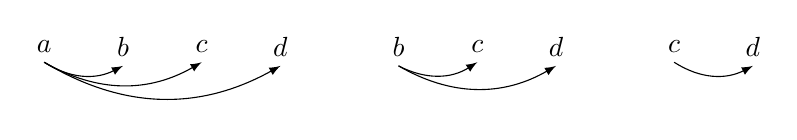
\begin{tikzpicture}[>=latex,scale=1.0]
  \begin{scope}
    \node (a1) at (-1.5,0){$a$};
    \node (b1) at (-0.5,0){$b$};
    \node (c1) at (0.5,0) {$c$};
    \node (d1) at (1.5,0) {$d$};
    \draw[->](a1.south)to[bend right](b1.south);
    \draw[->](a1.south)to[bend right](c1.south);
    \draw[->](a1.south)to[bend right](d1.south);
  \end{scope}
  \begin{scope}[xshift=3.5cm]
    \node (b2) at (-0.5,0){$b$};
    \node (c2) at (0.5,0) {$c$};
    \node (d2) at (1.5,0) {$d$};
    \draw[->](b2.south)to[bend right](c2.south);
    \draw[->](b2.south)to[bend right](d2.south);
  \end{scope}
  \begin{scope}[xshift=6cm]
    \node (c3) at (0.5,0) {$c$};
    \node (d3) at (1.5,0) {$d$};
    \draw[->](c3.south)to[bend right](d3.south);
  \end{scope}
\end{tikzpicture}
\end{document}